\documentclass[10pt,draft]{article}

\usepackage{verbatim,multicol,color,amsmath,ifdraft, graphicx, wrapfig,setspace}

%\usepackage[latin1]{inputenc}
%\usepackage[T1]{fontenc}
%\usepackage[dvips]{graphicx}

\title{STAT 401A Mid-term Exam \\ Friday 24 February 8:00-8:50}
\author{Instructor: Jarad Niemi}
\date{}

\newenvironment{longitem}{
\begin{itemize}
  \setlength{\itemsep}{15pt}
  \setlength{\parskip}{20pt}
  \setlength{\parsep}{20pt}
}{\end{itemize}}

\setlength{\textheight}{9in}
\setlength{\textwidth}{6.5in}
\setlength{\topmargin}{-0.125in}
\setlength{\oddsidemargin}{-.2in}
\setlength{\evensidemargin}{-.2in}
\setlength{\headsep}{0in}

\newcommand{\bigbrk}{\vspace*{2in}}
\newcommand{\smallbrk}{\vspace*{.3in}}

\ifdraft{
  \newcommand{\correct}[1]{{\color{red} #1}}
  \newcommand{\shortcorrect}[1]{{\color{red} #1}}
  \newcommand{\longcorrect}[2][\bigbrk]{{\color{red} #2}}
}{
  \newcommand{\correct}[1]{\underline{\phantom{XXXXXX}}}
  \newcommand{\shortcorrect}[1]{{\phantom{33.33}}}
  \newcommand{\longcorrect}[2][\bigbrk]{#1}
}

\newcommand{\iid}{\stackrel{iid}{\sim}}
\newcommand{\Yiid}{Y_1,\ldots,Y_n\stackrel{iid}{\sim}}

\begin{document}

\maketitle


\bigskip


\textbf{INSTRUCTIONS}

Please check to make sure you have 5 pages with writing on the front and back except for the very last page which is blank.

\bigskip

On the following pages you will find short answer questions related to the topics we covered in class for a total of 50 points. Please read the directions carefully.

\bigskip

You are allowed to use a calculator and one $8\frac{1}{2}\times 11$ sheet of paper with writing on both front and back. A non-exhaustive list of items you are not allowed to use are {\bf cell phones, laptops, PDAs, and textbooks}. Cheating will not be tolerated. Anyone caught cheating will receive an automatic F on the exam. In addition the incident will be reported, and dealt with according to University's Academic Dishonesty regulations. Please refrain from talking to your peers, exchanging papers, writing utensils or other objects, or walking around the room. All of these activities can be considered cheating. {\bf If you have any questions, please raise your hand.}

\bigskip

You will be given only the time allotted for the course, no extra time will be given.

\bigskip

Some notation that should be familiar:
\begin{center}
\begin{tabular}{ll}
%$Exp(\beta)$ &: exponential distribution with mean $\beta$ \\
%$Be(\alpha,\beta)$ &: beta distribution with parameters $\alpha$ and $\beta$ \\
%$Geo(p)$ &: Geometric distribution with probability of success $p$ \\
$t_v$ &: $t$-distribution with $v$ degrees of freedom \\
%$\chi^2_v$ &: $\chi^2$-distribution with $v$ degrees of freedom \\
$F_{u,v}$ &: $F$-distribution with $u$ numerator and $v$ denominator degrees of freedom \\
\hline
%$\chi^2_{v,\alpha}$ &: the value $c$ such that $P(X>c)=\alpha$ if $X\sim \chi^2_v$ \\
$t_{v}(a)$ &: the value $c$ such that $P(X<c)=a$ if $X\sim t_v$ \\
%$z_{\alpha}$ &: the value $c$ such that $P(X>c)=\alpha$ if $X\sim N(0,1)$ \\
\hline
$\overline{y}$ &= $\frac{1}{n} \sum_{i=1}^n y_i$ \\
$s_y^2$ &= $\frac{1}{n-1} \sum_{i=1}^n (y_i-\overline{y})^2$ \\
\end{tabular}
\end{center}

\smallbrk

Good Luck!

\smallbrk

Please print your name below:

\smallbrk


Student Name: \underline{\phantom{XXXXXXXXXXXXXXXXXXXXXXXXXXXXXXXXXXXXXXXXX}}  


\begin{comment}
\newpage

\noindent \begin{Large}Mid-term peer evaluation  (10 pts total) \end{Large}
%\subsubsection*{Mid-term peer evaluation (10 pts for appropriately answering this question)} 

\bigskip

Please assign scores that reflect how you really feel about the extent to which the other members of your team contributed to your learning and/or your team's performance. This will be your only opportunity to reward the members of your team who worked hard on your behalf. (Note: If you give everyone pretty much the same score you will be hurting those who did the most and helping those who did the least.)

{\bf Instructions:} In the space below please rate each of the {\bf other} members of your team. Each member's peer evaluation score will be the average of the points they receive from the other members of the team. To complete the evaluation you should: 1) List the name of each member of your team in the alphabetical order of their last names and, 2) assign an average of ten points to the {\bf other} members of your team (Thus, for example, you should assign a total of 50 points in a six-member team; 60 points in a seven-member team; etc.) and, 3) differentiate some in your ratings; for example, you must give at least one score of 11 or higher (maximum=15) and one score of 9 or lower.

\vspace{0.2in}

\begin{tabular}{l@{\qquad\quad}c@{\qquad\qquad}c@{\qquad\qquad}l@{\qquad\qquad\quad}c@{\qquad\qquad}c@{\qquad\qquad}}
& Team Members & Score & & Team Members & Score \\
\hline
1) & & & 5) & & \\
\hline
2) & & & 6) & & \\
\hline
3) & & & 7) & & \\
\hline
4) & & & 8) & & \\
\hline
\end{tabular}


\vspace{0.3in}

{\bf Additional Feedback:} In the space below would you also briefly describe your reasons for your highest and lowest ratings. These comments -- but not information about who provided them -- will be used to provide feedback to students who would like to receive it.

Provide at least {\bf one positive critique} and {\bf one area for improvement}.

\vspace{0.2in}

{\bf Positive critiques:}

\vspace{2in}

{\bf Areas of improvment:} 

\end{comment}

\newpage

\noindent \begin{Large}Fill in the blank (10 pts total) \end{Large}

\bigskip

One point will be awarded for a correct answer in each blank. 

\bigskip

\begin{doublespace}
\begin{large}

\begin{longitem}
\item A p-value for a t-test is the probability of observing a t-ratio \correct{as or more extreme} than the t-statistic if the \correct{null hypothesis} is true.
\item Statistical inferences of cause-and-effect relationships can be drawn from  \correct{randomized experiments}. 
\item Inferences to populations can be drawn from \correct{random sampling}, but not otherwise. 
\item To perform all pairwise comparisons of means in an ANOVA model, the appropriate multiple comparison adjustment is the \correct{Tukey-Kramer} procedure.
\item To perform the Bonferroni correction on $k$ individual comparisons at an overall error rate of $\alpha$, the appropriate error rate for each individual test is \correct{$\alpha/k$}. 
\item Name 3 of the 4 assumptions in linear regression:

\vspace{-0.2in}

	\begin{itemize}
	\item \correct{Linearity}
	\item \correct{Normality}
	\item \correct{Constant variance}
	\item \correct{Independence}
	\end{itemize}
\item The $R^2$ statistic, or coefficient of determination, is the percentage of the \correct{total response variation} explained by the explanatory variable. 
\end{longitem}

\end{large}
\end{doublespace}

\newpage

\noindent \begin{Large}Test Selection  (10 pts total) \end{Large}

\bigskip 

\noindent For each row of graphs, please indicate the most appropriate test of equality of means/locations between the two samples. The possible responses are two-sample $t$-test, paired $t$-test, Welch's $t$-test, rank-sum test, and signed rank test. Each response should be used exactly once. On each histogram, the best fitting normal probability density function (bell-curve) is also shown. (2 pts each)

\vspace{0.2in}

\begin{minipage}{0.6\linewidth}
    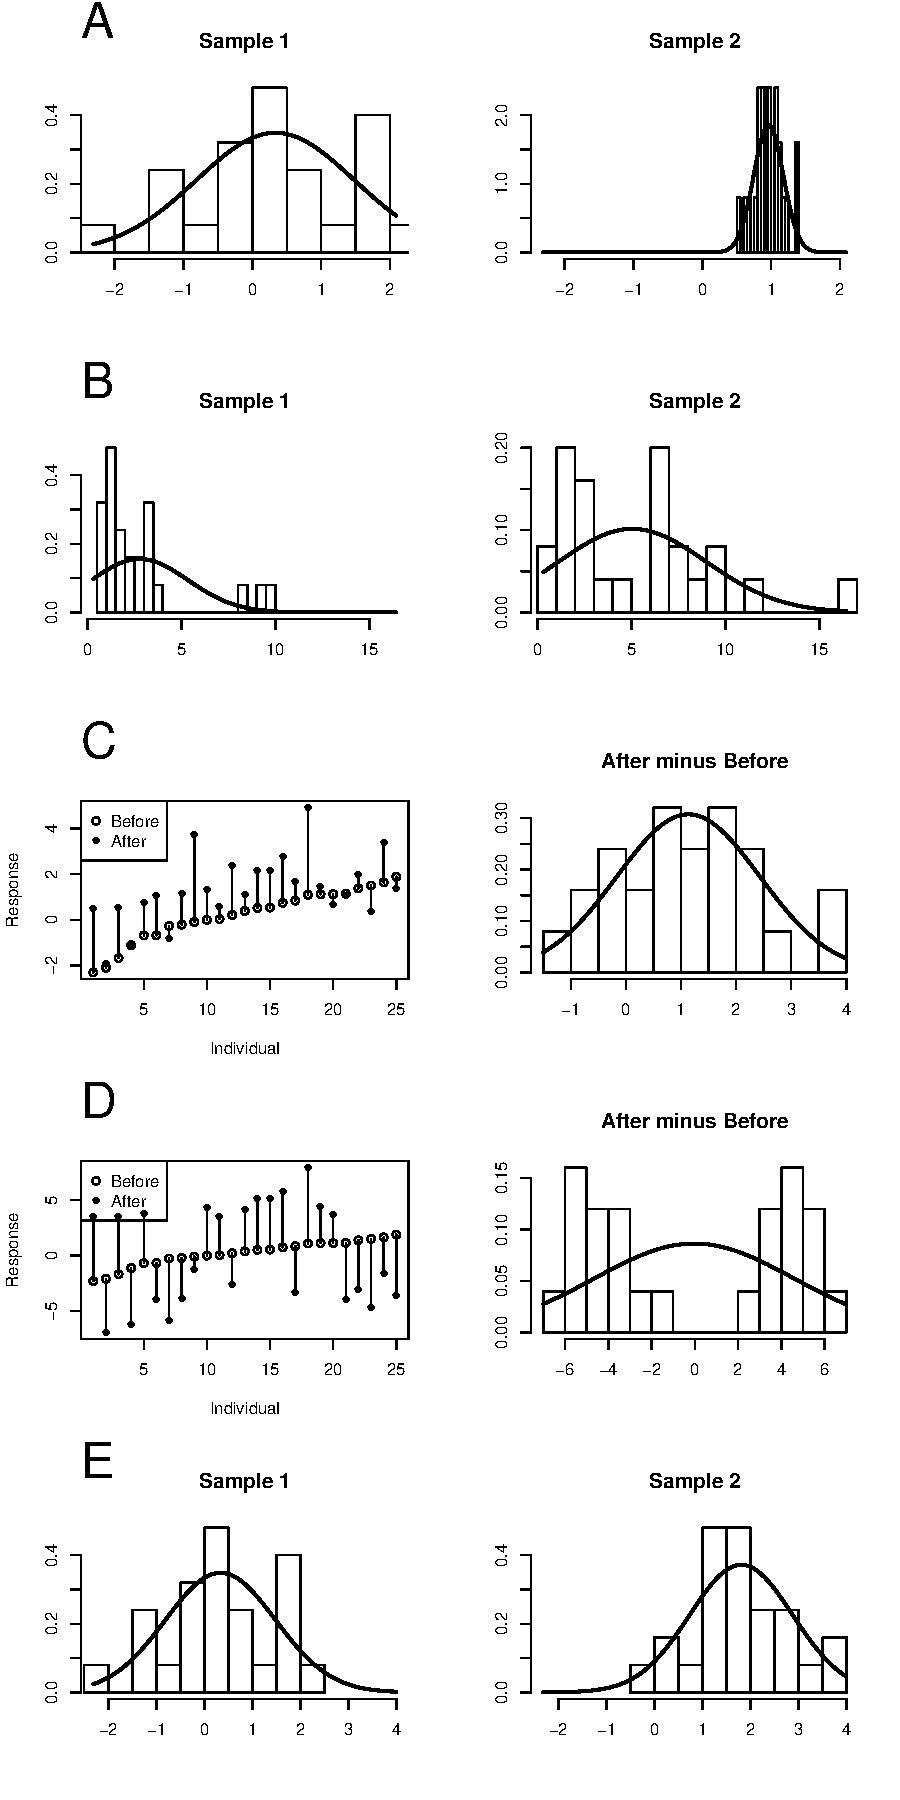
\includegraphics[width=\textwidth]{plots2}
\end{minipage}
\begin{minipage}{0.4\linewidth}
{\Huge

\vspace{-0.2in}

A.\correct{Welch's t-test}

\vspace{1.2in}

B.\correct{Rank-sum test}

\vspace{1.2in}

C.\correct{Paired t-test}

\vspace{1.2in}

D.\correct{Signed-rank test}

\vspace{1.2in}

E.\correct{Two-sample t-test}
}
\end{minipage}



\newpage
\noindent \begin{Large}Nematode lifespans (10 pts total) \end{Large}

\bigskip

Please answer the following questions {\bf based on the SAS code} titled ``Nematode lifespan''.

\begin{enumerate}
\item How many total data points are used in this analysis? (1 pt)

\shortcorrect{200}

\item How many groups are used in this analysis? (1 pt)

\shortcorrect{4} 

\item In statistical notation, what is the model used in this analysis ? (3 pts)\\
(Note: be sure to define any notation you introduce)

\longcorrect{\[Y_{ij}\stackrel{ind}{\sim} N(\mu_i,\sigma^2)\] where $Y_{ij}$ represents the lifespan of individual $j$ from group $i$.} 

\item Relative to the model in part c), what are the null and alternative hypotheses? (3 pts) 

\longcorrect{$H_0:\mu_i=\mu\mbox{ for all } i$ and $H_a:\mu_i\ne \mu_k$ for some $i\ne k$}

\item Provide a scientific conclusion based on the SAS output. (2 pts)

\longcorrect{We rejection the null hypothesis of a common mean lifespan amongst all treatments ($p<0.0001$).}

\end{enumerate}


\newpage
\noindent \begin{Large}Mercury in fish  (10 pts total) \end{Large}

\bigskip

\noindent The linear regression model states 
\[ Y_i \stackrel{ind}{\sim} N(\beta_0+\beta_1 X_i,\sigma^2). \]
Please answer the following questions {\bf based on the SAS code} titled ``Mercury in fish''.

\begin{enumerate}
\item What does $Y_i$ represent? (1 pt)

\shortcorrect{The mercury in ppm for fish $i$.}

\item What does $X_i$ represent? (1 pt)

\shortcorrect{The deviation (difference) from average weight in kilograms for fish $i$.} 

\item Provide an interpretation for $\beta_0$ including point estimate and 95\% confidence interval. (3 pts)

\longcorrect{
\begin{align*}
t_{170}(.975) &\approx 1.98 \\
95\% CI &= 1.19180 \pm 1.98\cdot 0.04864 = (1.10,1.29)
\end{align*}
At the mean weight (1.148kg), the expected mercury in ppm is 1.19 with 95\% CI (1.10,1.29).
}

\item Provide an interpretation for $\beta_1$ including point estimate and 95\% confidence interval. (3 pts)

\longcorrect{
\begin{align*}
95\% CI &= 0.48181 \pm 1.98\cdot 0.05572 = (0.37,0.59)
\end{align*}
For each kilogram increase in fish weight, the expected increase in mercury in ppm is 0.48 with a 95\% CI of (0.37,0.59).
}

\item Provide a point estimate and 95\% prediction interval for the amount of mercury in a fish weighing 2.148kg. (Hint: SXY=62.8) (2 pts)

\longcorrect{
\begin{align*}
X_0 &= 2.148-1.148=1 \\
Y_0 &= 1.1918+.48181(1)= 1.67361\\
SXX &= SXY/\hat{\beta}_1 = 62.8/.48181 = 130 \\
SE(Pred\{Y|X_0\}) &= \hat{\sigma}\sqrt{1+\frac{1}{n} + \frac{(X_0-\overline{X})^2}{SXX}}= \hat{\sigma}\sqrt{1+\frac{1}{171} + \frac{1}{130}} = 0.64\\
\end{align*}
A 95\% prediction interval is $1.67361\pm 1.98 (.64) = (0.41,2.94)$
}

\end{enumerate}

\newpage
Problem \#3 - SAS code for Nematode lifespan
\begin{verbatim}
title 'Nematode lifespan';
data life;
  infile 'NematodeLifespan.csv' delimiter=',' firstobs=2;
  input treatment $ lifespan;
  run;

proc glm data=life;
  class treatment;
  model lifespan = treatment;
  run; quit;


                                        Nematode lifespan    

                                        The GLM Procedure

Dependent Variable: lifespan

                                               Sum of
       Source                      DF         Squares     Mean Square    F Value    Pr > F

       Model                        3     1617.120000      539.040000      15.25    <.0001

       Error                      196     6928.000000       35.346939

       Corrected Total            199     8545.120000


                      R-Square     Coeff Var      Root MSE    lifespan Mean

                      0.189245      31.92980      5.945329         18.62000
 \end{verbatim}

\newpage
Problem \# 4 - SAS code for Mercury in fish
\begin{verbatim}
title 'Mercury in fish';
data boulder;
  infile 'fish.csv' delimiter=',' firstobs=2;
  input river station length weight mercuryPPM;
  weightKG = weight/1000;
  centered = weightKG - 1.148; /* mean weight in kilograms is 1.148 */
  run;

proc reg;
  model mercuryPPM=centered;
  run;


                                        Mercury in fish  

                                 Dependent Variable: mercuryPPM

                                      Analysis of Variance

                                             Sum of           Mean
         Source                   DF        Squares         Square    F Value    Pr > F

         Model                     1       30.25105       30.25105      74.77    <.0001
         Error                   169       68.37122        0.40456
         Corrected Total         170       98.62227


                      Root MSE              0.63605    R-Square     0.3067
                      Dependent Mean        1.19175    Adj R-Sq     0.3026
                      Coeff Var            53.37115


                                       Parameter Estimates

                                    Parameter       Standard
              Variable      DF       Estimate          Error    t Value    Pr > |t|

              Intercept      1        1.19180        0.04864      24.50      <.0001
              centered       1        0.48181        0.05572       8.65      <.0001
\end{verbatim}


\end{document}

